%Sección 4.1
\subsection{Etapa 1: Planeación}\label{subsec:Planeacion}

En esta etapa, se estableció el propósito general de la investigación y se definieron las metas, así como las preguntas de investigación,
métricas, criterios de clasificación, criterios de inclusión/exclusión y criterios de calidad de los estudios. Ver Figura~\ref{fig:etapa1}.

\begin{figure}[htbp]
        \centering
        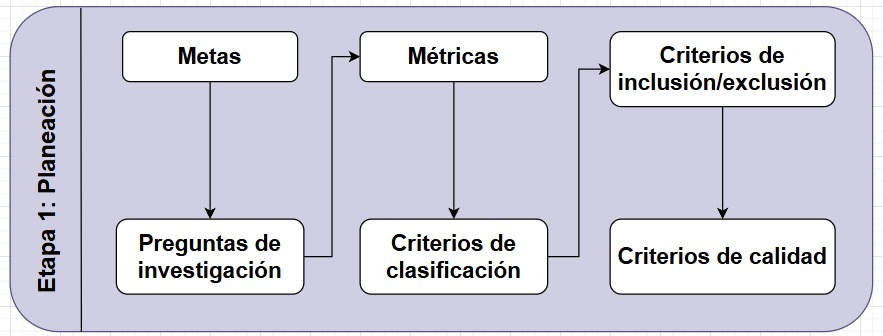
\includegraphics[width=0.5\textwidth]{resources/images/Planeacion/Etapa_1.jpeg}
        \caption{Composición de la etapa de planeación}\label{fig:etapa1}
\end{figure}

\subsubsection{Objetivos}
Teniendo en cuenta los aspectos descritos en la sección de motivación~\ref{sec:Motivacion}, se definieron 2 metas generales para la 
revisión sistemática de la literatura que se presentan en el cuadro~\ref{tab:metas}.

\begin{table}[htbp]
    \centering
    \begin{tabular}{>{\centering\arraybackslash}m{0.5cm}>{\arraybackslash}m{7cm}}
        \hline
        \textbf{Metas} & \textbf{Descripción} \\
        \hline\\
        M1 & Identificar trabajos relacionados con la seguridad de la información en entornos de computación en la nube, según su enfoque, mecanismos de protección, gestión de riesgos y examinando su grado de alineación con estándares internacionales de referencia, tales como las normas ISO/IEC 27001, 27017 y 27018, en contextos institucionales de investigación. \\
        \\
        M2 & Determinar una estructura de clasificación de trabajos que aborden la seguridad de la información en la computación en la nube como soporte para las funciones universitarias de investigación, docencia y gestión institucional. \\\\
        \hline
        \vspace{1pt}
    \end{tabular}
    \caption{Metas del estudio}\label{tab:metas}
\end{table}

\subsubsection{Pregunta de investigación}
Para la construcción de las preguntas de investigación (RQ, por sus siglas en inglés) se utilizó GQM \textit{(Goal Question Metric)}~\cite{Needleman2002} y el modelo PICOC~\cite{petticrew2008systematic}.
Este modelo permite establecer aspectos como ``Población'', ``Intervención'', ``Comparación'', ``Salida'' y ``Contexto'' que sirven para situar el trabajo a realizar.
Ver cuadro~\ref{tab:PICOC}.


\begin{table}[tbp]
    \scriptsize % reduce tamaño del texto
    \centering
    \renewcommand{\arraystretch}{1.0}
    \begin{tabularx}{\columnwidth}{>{\centering\arraybackslash}m{0.18\columnwidth} >{\raggedright\arraybackslash}X}
        \hline
        \textbf{Aspecto} & \textbf{Descripción} \\
        \hline
        Población & Estudios relacionados a las buenas prácticas, normativas, controles y marcos de referencias internacionales para la seguridad de la computación en la nube. \\
        Intervención &
        1. Identificación de un conjunto de buenas prácticas, controles, metodologías, herramientas y tecnologías.~\newline
        2. Identificar el modelo taxonómico de los trabajos. \\
        Comparación &
        1. Estudios que han hecho uso de normas internacionales para la seguridad de la información de la computación de la nube y que se demuestre mayor tasa de éxito en contrarrestar ataques informáticos.~\newline
        2. Se examina la importancia de la ciberseguridad y su impacto en trabajos de docencia, investigación y la gestión institucional.~\newline
        3. Se aplican criterios de inclusión y exclusión. \\
        Salida & Documentos y estructura de clasificación sobre arquitecturas de seguridad relacionados con las normativas internacionales que han impactado en proyectos de docencia, investigación y gestión institucional. \\
        Contexto & Gestión institucional, seguridad de la computación en la nube, confidencialidad, integridad y disponibilidad de servicios en la nube. \\
        \hline
        \vspace{1pt}
    \end{tabularx}
    \caption{Aspectos del modelo PICOC}\label{tab:PICOC}
\end{table}

Teniendo en cuenta la información del modelo PICOC, se definieron 2 RQ.\@ Ver cuadro~\ref{tab:preguntas}.

\begin{table*}[!t]
    \centering
    \renewcommand{\arraystretch}{1.4}
    \begin{tabularx}{\textwidth}{>{\centering\arraybackslash}m{0.02\textwidth} >{\centering\arraybackslash}m{0.04\textwidth} >{\raggedright\arraybackslash}X >{\raggedright\arraybackslash}X}
    \toprule
    \textbf{Meta} & \textbf{Pregunta} & \textbf{Descripción} & \textbf{Motivación} \\
    \midrule
    G1 & Q1 & ¿Qué trabajos abordan arquitecturas de seguridad en entornos de computación en la nube para contextos institucionales y universitarios, y qué enfoques de protección de activos, gestión de riesgos y controles de seguridad proponen, en relación con estándares y buenas prácticas internacionales? & Sobre las arquitecturas de seguridad en entornos de computación en la nube, alineadas con los controles de las normas ISO/IEC 27001, 27017 y 27018 y demás estándares internacionales y su impacto en contextos institucionales y universitarios: \newline
    1. Reconocer cómo las arquitecturas de seguridad en la nube apoyan la protección de la información en procesos de investigación, docencia y gestión académica.~\newline
    2. Identificar los mecanismos, controles y componentes de seguridad utilizados en las arquitecturas analizadas.~\newline
    3. Determinar el contexto y propósito de aplicación de las arquitecturas consideradas. \\
    \midrule
    G2 & Q2 & ¿Cuál es la estructura taxonómica de las arquitecturas de seguridad en la computación en la nube que contribuyen al fortalecimiento de funciones institucionales en entornos universitarios, tales como la investigación, la docencia y la gestión institucional? & Sobre las arquitecturas de seguridad en la computación en la nube aplicadas a entornos universitarios y su contribución al fortalecimiento de funciones institucionales: \newline
    1. Reconocer cómo se clasifican las arquitecturas de seguridad propuestas en la literatura para la protección de activos de información en la nube.~\newline
    2. Identificar el aporte de los controles de seguridad y mecanismos implementados en las arquitecturas evaluadas.~\newline
    3. Determinar el impacto de estas arquitecturas en la mejora de la gestión tecnológica y administrativa dentro de instituciones de educación superior. \\
    \bottomrule
    \vspace{1pt}
    \end{tabularx}
    \caption{Preguntas de investigación y su motivación}\label{tab:preguntas}
\end{table*}

\subsubsection{Métricas}

Se establecieron las métricas del estudio mediante un enfoque cuantitativo, conforme a la estructura de clasificación. Los detalles de 
dichas métricas se presentan en el cuadro~\ref{tab:metricas}. Los criterios definidos limitaron la validez de los documentos a un periodo 
de tres años, con el fin de favorecer la actualidad del estudio. Asimismo, el tipo de fuente se restringió a estudios primarios, con el 
propósito de asegurar un mayor rigor en la revisión por pares.

\begin{table}[htbp]
    \centering
    \renewcommand{\arraystretch}{1.3}
    \begin{tabularx}{\columnwidth}{>{\centering\arraybackslash}m{0.06\textwidth} >{\raggedright\arraybackslash}X}
    \toprule
    \textbf{Métrica} & \textbf{Descripción} \\
    \midrule
    M1 & Cantidad de trabajos referentes a  metodologías, marcos de referencia y buenas prácticas  de la seguridad de la computación en la nube. \\
    M2 & Cantidad de trabajos con referentes de herramientas tecnológicas y tecnologías relacionados con la seguridad de la computación en la nube. \\
    M3 & Cantidad de trabajos relacionados con casos de estudio referentes a la seguridad de la computación en la nube. \\
    M4 & Cantidad de trabajos referentes al fortalecimiento de la seguridad en la computación en la nube en funciones institucionales de entornos universitarios. \\
    \bottomrule
    \vspace{1pt}
    \end{tabularx}
    \caption{Métricas definidas para el análisis}\label{tab:metricas}
\end{table}

\subsubsection{Tópicos de investigación}

Las preguntas de investigación y el modelo PICOC sirven como línea base para definir los tópicos considerados relevantes en el estudio.
Los tópicos definidos para cada pregunta fueron los siguientes:

\begin{itemize}
    \item \textbf{Q1:} \textit{Security}, \textit{ISO/IEC 27001}, \textit{Architecture}, \textit{Security Controls}, \textit{Cloud Computing}, \textit{Cybersecurity}, \textit{SECURITY INFORMATION AND EVENT MANAGEMENT (SIEM)}.

    \item \textbf{Q2:} \textit{Classification}, \textit{Architecture}, \textit{Taxonomy}, \textit{Cloud Computing}, \textit{Security}, \textit{ZERO-TRUST}.
\end{itemize}

La definición de los tópicos de investigación se realizó considerando los dominios conceptuales más relevantes asociados a cada pregunta de investigación.\\

\subsubsection{Criterios de inclusión y exclusión}
\mbox{}\\
\begin{table*}[!t]
    \centering
    \renewcommand{\arraystretch}{1.0}
    \begin{tabularx}{\textwidth}{>{\centering\arraybackslash}m{0.15\textwidth} >{\raggedright\arraybackslash}X >{\raggedright\arraybackslash}X}
    \toprule
    \textbf{Categoría} & \textbf{Inclusión} & \textbf{Exclusión} \\
    \midrule
    Campos & Resumen, titulo y palabras clave & --- \\
    \midrule
    Tipo de publicación & Artículos y capitulos publicados en revistas científicas o académicas y actas de congresos & Informe técnico, actas de congresos y tesis. \\
    \midrule
    Área/Disciplina & Administración, Informática, Tecnologías de la Información y Ciberseguridad. & Áreas no relacionadas con la gestión, Informática, Tecnologías de la Información y Ciberseguridad. \\
    \midrule
    Período & Entre 2020 to 2026 & Menos de 2020 \\
    \midrule
    Idioma & Inglés & --- \\
    \bottomrule
    \vspace{1pt}
    \end{tabularx}
    \caption{Criterios de inclusión y exclusión}\label{tab:criterios}
\end{table*}
Los criterios de inclusión y exclusión se definieron con el fin de garantizar que los estudios seleccionados fueran pertinentes para 
responder a las preguntas de investigación y cumplir con los objetivos del estudio. Dichos criterios se presentan en la Tabla~\ref{tab:criterios}.
En primer lugar, se consideraron únicamente los campos de título, resumen y palabras clave para la identificación inicial de los estudios. 
En cuanto al tipo de publicación, se incluyeron artículos y capítulos publicados en revistas científicas, académicas y en actas de 
congresos, mientras que se excluyeron informes técnicos y tesis. Respecto al área o disciplina, se incluyeron estudios pertenecientes a 
los campos de Administración, Informática, Tecnologías de la Información y Ciberseguridad, excluyendo aquellos que no estuvieran 
relacionados con estas áreas. Asimismo, se estableció un período de publicación comprendido entre los años 2020 y 2026, con el objetivo de 
priorizar estudios recientes y reflejar el estado actual de la investigación en el área. Finalmente, se consideraron únicamente estudios 
escritos en inglés, con el propósito de asegurar la accesibilidad y comparabilidad de la literatura analizada.

\subsubsection{Criterios de calidad}\label{subsec:criterios_calidad}

Para finalizar la etapa de planeación, se definieron tres criterios de calidad. \\

El primer criterio de calidad es una adaptación del CVI \textit{(Content Value Index)}.
En este caso, los artículos se evaluaron para determinar si cumplen con los criterios de inclusión y exclusión definidos y si son relevantes
para las preguntas de investigación. Se usó una escala cuantitativa de 0 a 5, donde 0 indica una baja relación con las metas del SMS y 5 
indica una alta relación. Ver formula~\ref{eq:cvi}. En esta formula, \textbf{K} es el número impar de evaluadores y \textbf{\textit{f (n)}} 
es la frecuencia de respuestas para cada valor de la escala.\\

\begin{equation}
    \label{eq:cvi}
    CVI = \frac{\sum_{n=1}^{k} f(n)}{k}
\end{equation}

El segundo criterio de calidad es el número de citas de cada estudio de acuerdo con la fecha de publicación (\textbf{A}), el cual se 
denomina SCI \textit{(Scientific Citation Index)}. Ver formula~\ref{eq:sci}. En esta formula, \textbf{C} es el número de citas entre 2022 y 
2024 y \textbf{A} es el tiempo de publicación del estudio. Así, un artículo publicado en 2024 con las misma cantidad de citas que un 
artículo publicado en 2022 tendrá un SCI más alto.\\

\begin{equation}
    \label{eq:sci}
    SCI = \frac{C}{A}
\end{equation}

El tercer criterio de calidad corresponde a la relación de los estudios con las preguntas de investigación. Este criterio se denomina 
IRRQ \textit{(Index of Relationship to Research Questions)}. Ver formula~\ref{eq:irrq}.

\begin{equation}
    \label{eq:irrq}
    IRRQ = \frac{N}{2}
\end{equation}

\textbf{N} corresponde al número de preguntas de investigación que el estudio responde. Este valor se divide en 2 porque es el número de 
preguntas de investigación definidas en la etapa de planeación.\\